\documentclass[12pt]{exam}

\usepackage{amssymb}
\usepackage{mathtools}
\usepackage{algorithm}
\usepackage{float}  % Figure placement
\usepackage{minted}  % Code highlighting
\usepackage{tikz}  % Flow chart
\usepackage{lipsum}
\usepackage{xspace}
\usepackage{hyperref}
\usepackage{MnSymbol}
\usepackage{pgffor}
\usepackage{mdframed}


\hypersetup{
    colorlinks = true,
    linkcolor = blue,
    urlcolor  = blue,
    citecolor = blue,
    anchorcolor = blue
}

\newcommand{\hwheaderfooter}[3]{
\pagestyle{headandfoot}
\firstpageheadrule
\firstpageheader{#1}{#2}{#3}
\runningheader{#1}{#2}{#3}
\runningheadrule
\firstpagefooter{}{\thepage}{}
\runningfooter{}{\thepage}{}
}

\newcommand{\latex}{\LaTeX\xspace}

\newcommand{\stars}[1]{%
    \foreach \n in {1,...,#1}{%
        $\filledstar$%
    }%
}




\hwheaderfooter{HW 1}{Ching}{CSCI 406}


\begin{document}
\begin{center}
    \fbox{\fbox{\parbox{\textwidth - 0.2 in}{\centering
                {Instructions: Please note that handwritten assignments \textbf{will not be graded}. Use the
                    provided \latex template to complete your homework. Please do not alter the order or spacing of
                    questions (keep each question on its own page). When you submit to Gradescope, you must mark
                    which page(s) correspond to each question. \textbf{You may not receive credit for unmarked
                        questions}. \\
                    When including graphical figures, we encourage the use of tools such as \href{https://dreampuf.github.io/GraphvizOnline/}{graphviz} or packages like \href{https://www.overleaf.com/learn/latex/TikZ_package}{tikz} for simple and complex figures. However, these may be handwritten only if they are neat and legible (as defined by the grader). } \\
                \hrulefill\par\nobreak\hskip - \leftskip\bfseries
                All answers must be \textbf{concise and complete}. See the Homework Guide for tips on how to write concise and complete answers.
            }}}
\end{center}

\begin{questions}

    \question For the following questions, select whether the statement is true or false,
    and write a \textit{brief} explanation of your reasoning.

    \begin{parts}
        \part[4] [W2, \stars{1}] For undirected graphs, we really only need about half of an adjacency
        matrix to store the graph.

        % Replace \square with \blacksquare for the option you would like to select.
        $\blacksquare$ True $\square$ False

        This is because the matrix is symmetric and the diagonal is all 0, so we only need to store the upper or lower triangle.

        \part[4] [W2, \stars{1}]
        Adjacency matrices allow one to quickly iterate through all the edges
        of a particular node, while adjacency lists allow us to check in constant time
        if two nodes are adjacent.

        % Replace \square with \blacksquare for the option you would like to select.
        $\square$ True $\blacksquare$ False

        Adjacency matrices are constant time to check if two nodes are connected.
        Adjacency lists are linear time to iterate through list of connected nodes too check if two nodes are adjacent.

        \part[4] [W2, \stars{1}]
        Adjacency lists use memory much more efficiently than adjacency matrices for sparse graphs.

        % Replace \square with \blacksquare for the option you would like to select.
        $\blacksquare$ True $\square$ False

        Adjacency lists only store the edges that exist, while adjacency matrices store all possible edges (including non-existing connections).

        \part[4] [W2, \stars{1}] A BFS uses a queue data structure.

        % Replace \square with \blacksquare for the option you would like to select.
        $\blacksquare$ True $\square$ False \hspace{0.5in} \textbf{No explanation necessary for this problem.}

    \end{parts}

    \clearpage

    \question The following questions are related to the maze project. No explanation is necessary for these problems.

    \begin{parts}
        \part[5] [W2, \stars{1}] Select all the statements that are true.

        % Replace \square with \blacksquare for the options you would like to select.
        $\blacksquare$ If Captain Rocket is in a room colored \texttt{B}, Lieutenant Lucky can move along a corridor which is colored \texttt{B} outgoing from the room Lieutenant Lucky is currently in.

        $\square$ Captain Rocket and Lieutenant Lucky must alternate and each should move every-other turn.

        $\square$ Both Captain Rocket and Lieutenant Lucky must get to the Goal to solve the maze.

        $\blacksquare$ Each corridor has a single direction along which travel is possible.

        \part[2] [W2, \stars{1}] Select the true statement.

        % Replace \square with \blacksquare for the options you would like to select.
        $\square$ The graph traversal algorithm used in my project should be DFS.

        $\blacksquare$ The graph traversal algorithm used in my project should be BFS.

        $\square$ I need to create my own graph traversal algorithm to complete this project.

        \part[2] [W2, \stars{1}] In the input for the project, if you have the following line
        \begin{verbatim}
4 6 A
\end{verbatim}
        then there is a corridor from room 4 to room 6 with color \texttt{A}.

        % Replace \square with \blacksquare for the option you would like to select.
        $\blacksquare$ True $\square$ False

        \part[5] [W2, \stars{1}] If the first three lines of the input file are

        \begin{verbatim}
10 20
G R B R G B B R G R
4 7
\end{verbatim}
        select all the statements that are true.

        % Replace \square with \blacksquare for the options you would like to select.
        $\blacksquare$ There are 10 rooms and 20 corridors.

        $\square$ There are 20 rooms and 10 corridors.

        $\square$ Captain Rocket starts in room 7 and Lieutenant Lucky starts in room 4.

        $\blacksquare$ Captain Rocket starts in room 4 and Lieutenant Lucky starts in room 7.

        $\blacksquare$ There are three distinct colors: \texttt{G}, \texttt{R}, and \texttt{B}.

    \end{parts}

    \clearpage

    \question[10] [W2, \stars{2}]
    While working at a large Fortune 500 company, your CEO boasts ``even though
    our company is large, there are no more than 7 levels between me and any
    employee.'' Given the organizational hierarchy of the company, how can you
    verify the CEO's claim? (Your answer should be a few sentences at most.)

    This can be verified by:
    \begin{itemize}
        \item Use BFS to find the shortest path between the CEO and any employee.
        \item If any path is greater than 7, then the CEO's claim is false.
    \end{itemize}



    \clearpage

    \question[10] [W2, \stars{3}] Connected Components.
    \begin{parts}
        \part[5] Is it possible to draw an undirected, unweighted, simple graph with exactly 7 vertices, \textbf{11} edges, and 3 connected components? If so, then give the graph. If not, explain why it is not possible.

        No this is not possible. To achieve the 3 we need 2 vertices with no edges, and a complete graph with 5 vertices. This would give us 10 edges, so it is not possible. (See next question for example)

        \part[5] Is it possible to draw an undirected, unweighted, simple graph with exactly 7 vertices, \textbf{10} edges, and 3 connected components? If so, then give the graph. If not, explain why it is not possible.

        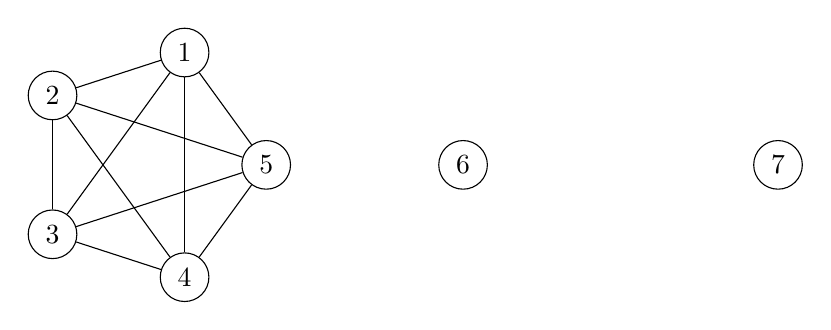
\begin{tikzpicture}
            % Nodes forming a complete graph
            \foreach \i in {1,...,5}
            \node[circle, draw] (N\i) at (72*\i:1.5) {\i};

            % Edges for the complete graph
            \foreach \i in {1,...,4}
            \foreach \j in {\i,...,5}
            \draw (N\i) -- (N\j);

            % Two additional nodes not linked to anything
            \node[circle, draw] (X1) at (4,0) {6};
            \node[circle, draw] (X2) at (8,0) {7};
        \end{tikzpicture}

    \end{parts}
    \clearpage

    \question[20] [W2, \stars{3}] Graph Coloring. Remember from class that a graph coloring is an assignment of colors to vertices such that no edge connects two vertices of the same color.

    A \textbf{complete graph} is a graph in which every node has an edge to every other node.

    \begin{parts}
        \part Is it possible to two-color a complete graph of arbitrary size?

        % Replace \square with \blacksquare for the option you would like to select.
        $\square$ Yes $\blacksquare$ No

        \part Provide a \textit{concise but complete} proof for your answer to (a).

        \textbf{Counterexample:} Complete graph of size 3 cannot be two-colored.
        If we color the first node red, then the other two nodes must be blue.
        However, the other two nodes are connected, so they cannot be the same color.

        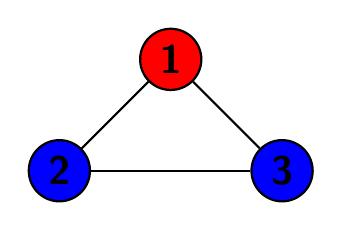
\begin{tikzpicture}[auto, node distance=2cm, every loop/.style={},
                thick,main node/.style={circle,draw,font=\sffamily\Large\bfseries}]

            % Nodes
            \node[main node, fill=red] (1) {1};
            \node[main node, fill=blue] (2) [below left of=1] {2};
            \node[main node, fill=blue] (3) [below right of=1] {3};

            % Edges
            \path[every node/.style={font=\sffamily\small}]
            (1) edge node {} (2)
            (1) edge node {} (3)
            (2) edge node {} (3);

        \end{tikzpicture}


        \part If it is not possible to two-color a complete graph of arbitrary size, then what is the minimum number of colors required to color a complete graph with $v$ vertices? Provide a \textit{concise but complete} proof. If it is possible to two-color a complete graph of arbitrary size, leave this question blank.

        \textbf{Claim:} For a complete graph $K_v$ with $v$ vertices, the required colors $\chi(K_v)$ is equal to the number of vertices $v$.

        \textbf{Proof:}

        \textit{Base Case:} For $v = 1$, the complete graph $K_1$ consists of a single vertex, and it trivially requires only one color. Thus, $\chi(K_1) = 1$.

        \textit{Inductive Step:} Assume that for a complete graph $K_n$, the chromatic number $\chi(K_n)$ is $n$. Now, consider adding a new vertex to form $K_{n+1}$.

        \begin{itemize}
            \item The new vertex is adjacent to all $n$ existing vertices in $K_n$.
            \item To color $K_{n+1}$, we need a new color for the newly added vertex since it is adjacent to all existing vertices.
            \item Therefore, $\chi(K_{n+1}) = n + 1$.
        \end{itemize}

        By induction, we have shown that the required colors of a complete graph with $v$ vertices ($K_v$) is equal to the number of vertices $v$, i.e., $\chi(K_v) = v$. Thus, the minimum number of colors required to color a complete graph with $v$ vertices is $v$.




    \end{parts}

    \clearpage

    \question[30] [W2, \stars{4}] Graph Modelling. Consider the following problem.
    \begin{mdframed}
        \textbf{University Scheduling}

        Consider a simplified university where each student takes exactly two courses. There are two time slots—morning and afternoon (that is, the student will have their morning course every morning, and their afternoon course every afternoon). Given the courses that each student has signed up for, determine if it is possible to teach each course exactly once (either in the morning or in the afternoon but not both) while satisfying all of the students course requirements.
    \end{mdframed}

    Provide a concise but complete description of how to model this problem as a graph and use an algorithm we have discussed in class to determine the answer. Be sure to describe how to interpret the result of the chosen algorithm to produce an answer to the problem.

    \textit{Note:} It is recommended to provide the answer to this question in a list of steps.

    \textbf{Create Graph:}
    \begin{enumerate}
        \item Create a vertex for each course.
        \item Create an edge for each student, connecting the two courses they are taking.
        \item Assign each vertex a binary color (morning or afternoon).
    \end{enumerate}

    \textbf{Algorithm:} Use DFS
    \begin{enumerate}
        \item Start at any vertex.
        \item Assign the vertex a color.
        \item Assign the adjacent vertices the opposite color.
        \item Repeat for all unvisited vertices.
        \item If a vertex is assigned a color that is the same as an adjacent vertex, then the graph is not 2-colorable.
        \item If all vertices are assigned a color, then the graph is 2-colorable.
    \end{enumerate}

    \textbf{Interpretation:} If the graph is 2-colorable, then it is possible to teach each course exactly once while satisfying all of the students course requirements. Otherwise, it is not possible.

    % close the document
\end{questions}
\end{document}
